\documentclass[a4paper, 12pt, twoside]{report}

%packagessss
            \usepackage[margin=1in]{geometry}
            \usepackage[table]{xcolor}
            \usepackage{amsmath}
            \usepackage{amssymb}
            \usepackage{graphicx}
            \usepackage[toc,page]{appendix}
            \usepackage[numbers]{natbib}
            \usepackage{chemformula}
            \usepackage{fancyhdr}
            \usepackage{lipsum}
            \usepackage{float}
            \usepackage{booktabs}
            \PassOptionsToPackage{hyphens}{url}\usepackage[hidelinks]{hyperref}
            \usepackage{multirow}
            \usepackage{caption}
            \usepackage{subcaption}
            \usepackage{array}
            \usepackage{setspace}
            \usepackage{titletoc}
            \usepackage{enumerate}
            \usepackage{mathptmx}
            \usepackage{fontspec}
            \setmainfont{Times New Roman}
            \setlength{\headheight}{15pt}
            \setstretch{1.20}

%important styles ====================================>
\newcolumntype{P}[1]{>{\centering\arraybackslash}p{#1}}

\titlecontents{chapter}
[0pt]
{\bfseries}
{\chaptername\ \thecontentslabel:\quad}
{}
{\hfill\contentspage}

\fancypagestyle{styletoc}{% 
\fancyhf{}
\fancyhead[LE,RO]{\textbf{\thepage}}
\fancyfoot{}
\renewcommand{\headrulewidth}{0.5pt}}

\fancypagestyle{stylenor}{% 
	\fancyhead[RE,LO]{\textbf{\leftmark}}
	\fancyhead[LE,RO]{\textbf{\thepage}}
    \fancyfoot{}
	\renewcommand{\headrulewidth}{0.5pt}}
\fancypagestyle{plain}{\pagestyle{fancy}}{}
%=================================================>

\begin{document}
%your title page ==================================>
\begin{titlepage}
\newgeometry{top=0.5in,left=0.2in,right=0.5in,bottom=1in}

\includegraphics[width = 50mm]{image/istic.png} \hfill
\begin{minipage}[b][3.00 \baselineskip]{20 em}
    \centering
    \textbf{République Tunisienne \\
    Ministère de l’Enseignement Supérieur \\
    et de la Recherche Scientifique \\
    Université de Carthage \\
    Institut Supérieur des Technologies de \\
    l’Information et de la Communication }
\end{minipage} \hfill  
\includegraphics[width = 0.20 \textwidth]{image/car.jpg}  
\vspace{1.5 cm}
\hrule

\vspace{3 cm}
\begin{center}
\LARGE{\textbf{Mini-Projet-web}}
\end{center}

\vspace{0.1 cm}
\begin{center}
\LARGE{\textbf{Rapport De Projet}}
\end{center}

\vspace{1.3 cm}
\hrule
\begin{center}
\huge{\textbf{Site Web Rissala}}
\end{center}
\hrule

\vspace{1.5 cm}
\begin{center}
\LARGE{\textbf{Membres}}
\end{center}

\vspace{0.1 cm}
\begin{center}
\Large{Ayoub Khefifi \\
Fedi Bellakhel  \\
Ahmed Akrout \\
Yassine chichti  }
\end{center}

\vspace{1.9 cm}
\hrule
\begin{center}
\Large{\textbf{Tutor:} \ \ \  Mme Sabrine Naimi} 
\end{center}

	\hrule
	\vspace{ 1 cm}
	\begin{center}
	\Large{\textbf{Date:} 16/02/2024}
	\end{center}
\end{titlepage}
%====================================================>

\shipout\null %empty page after title page if don't remove this line 

\pagenumbering{Roman} 
\pagestyle{styletoc}

%table of contents styles ============================>
\begin{doublespace}
\renewcommand*{\contentsname}{Table des matières}
\tableofcontents



\addcontentsline{toc}{chapter}{List of Tables}
\end{doublespace}

%your contents shows here:============================>



\pagenumbering{arabic}
\pagestyle{stylenor}

%chapters
\chapter{Introduction} 

%remove everything here ==============================>
\section{Introduction Generale : 
}
la dominance du contenu videographique absurde et sans valeur ajouté a été l'environnement ideal pour la naissance d'un nouveau format de contenu qui est
\section{les newsletters }
un court article ecrit par des createurs pour partager leurs connaissances et leurs experience. 
Dans ce cadre s'inscrit notre projet Rissala, qui est une plateforme de newsletters dédiée aux créateurs de contenu, leur permettant de partager leurs connaissances et leurs expériences par e-mail ou directement via leur profil sur Rissala.

\section{Qu'est-ce qu'une newsletter ?}
Les newsletters regroupent des articles offrant aux créateurs de contenu un moyen direct et personnel de rester en contact avec leur public. Elles les tiennent informés des dernières actualités, des nouveaux projets et leur permettent de partager des contenus exclusifs réservés aux abonnés, sans les contraintes d'une plateforme.
\section{Comment ça marche ?}
En s'abonnant à la newsletter d'un créateur de contenu, notre plateforme met à jour une base de données contenant leurs e-mails et envoie directement les articles créés par e-mail, tout en sauvegardant ces articles dans leur profil.
\section{Pourquoi une newsletter ?}
Une newsletter n'est pas soumise à des restrictions ni contrôlée par une plateforme, offrant ainsi aux créateurs de contenu la liberté de partager du contenu avec une audience ciblée et certainement intéressée.
\section{Le futur des newsletters :}
Face à la domination du contenu vidéographique et des contenus courts sur les réseaux sociaux, nous avons ressenti un besoin de relations directes et authentiques avec nos créateurs. L'absence de lectures, puisque de moins en moins de personnes lisent des livres, souligne l'importance des newsletters comme moyen d'adaptation. Ces articles, généralement de 2 à 8 pages, offrent une alternative engageante et informative dans un paysage numérique saturé 
\chapter{Diagramme du cas d'utilisation}


\section{Analyse Et Conception:}
Dans cette partie, nous utilisons la modélisation UML pour représenter les spécifications des
exigences grâce au diagramme de cas d’utilisation, mais aussi pour analyser le domaine avec le
diagramme de classe. Par la suite, nous abordons la conception, d’un point de vue fonctionnel,
technique et graphique. 
\section{Spécifications des exigences: Les cas d’utilisations}
Nous allons répondre aux questions suivantes : Quels sont les utilisateurs du système ? Quelles sont
leurs interactions avec celui-ci ? Il faut donc identifier les différents acteurs ainsi que les cas
d’utilisation c’est-à-dire les différentes fonctionnalités du système. 

\section{Les acteurs:}
\subsection{Admin : }
Une personne en charge de la gestion de la plateforme.
\subsection{Le créateur de contenu :}
Le protagoniste principal sur le site, bénéficiant du privilège de créer un compte, de publier et de gérer Rissala.
\subsection{Guest:}
Dans notre contexte, il s'agit de la personne qui consulte les newsletters et s'abonne au créateur de contenu.

\begin{figure}[p]
    \centering
    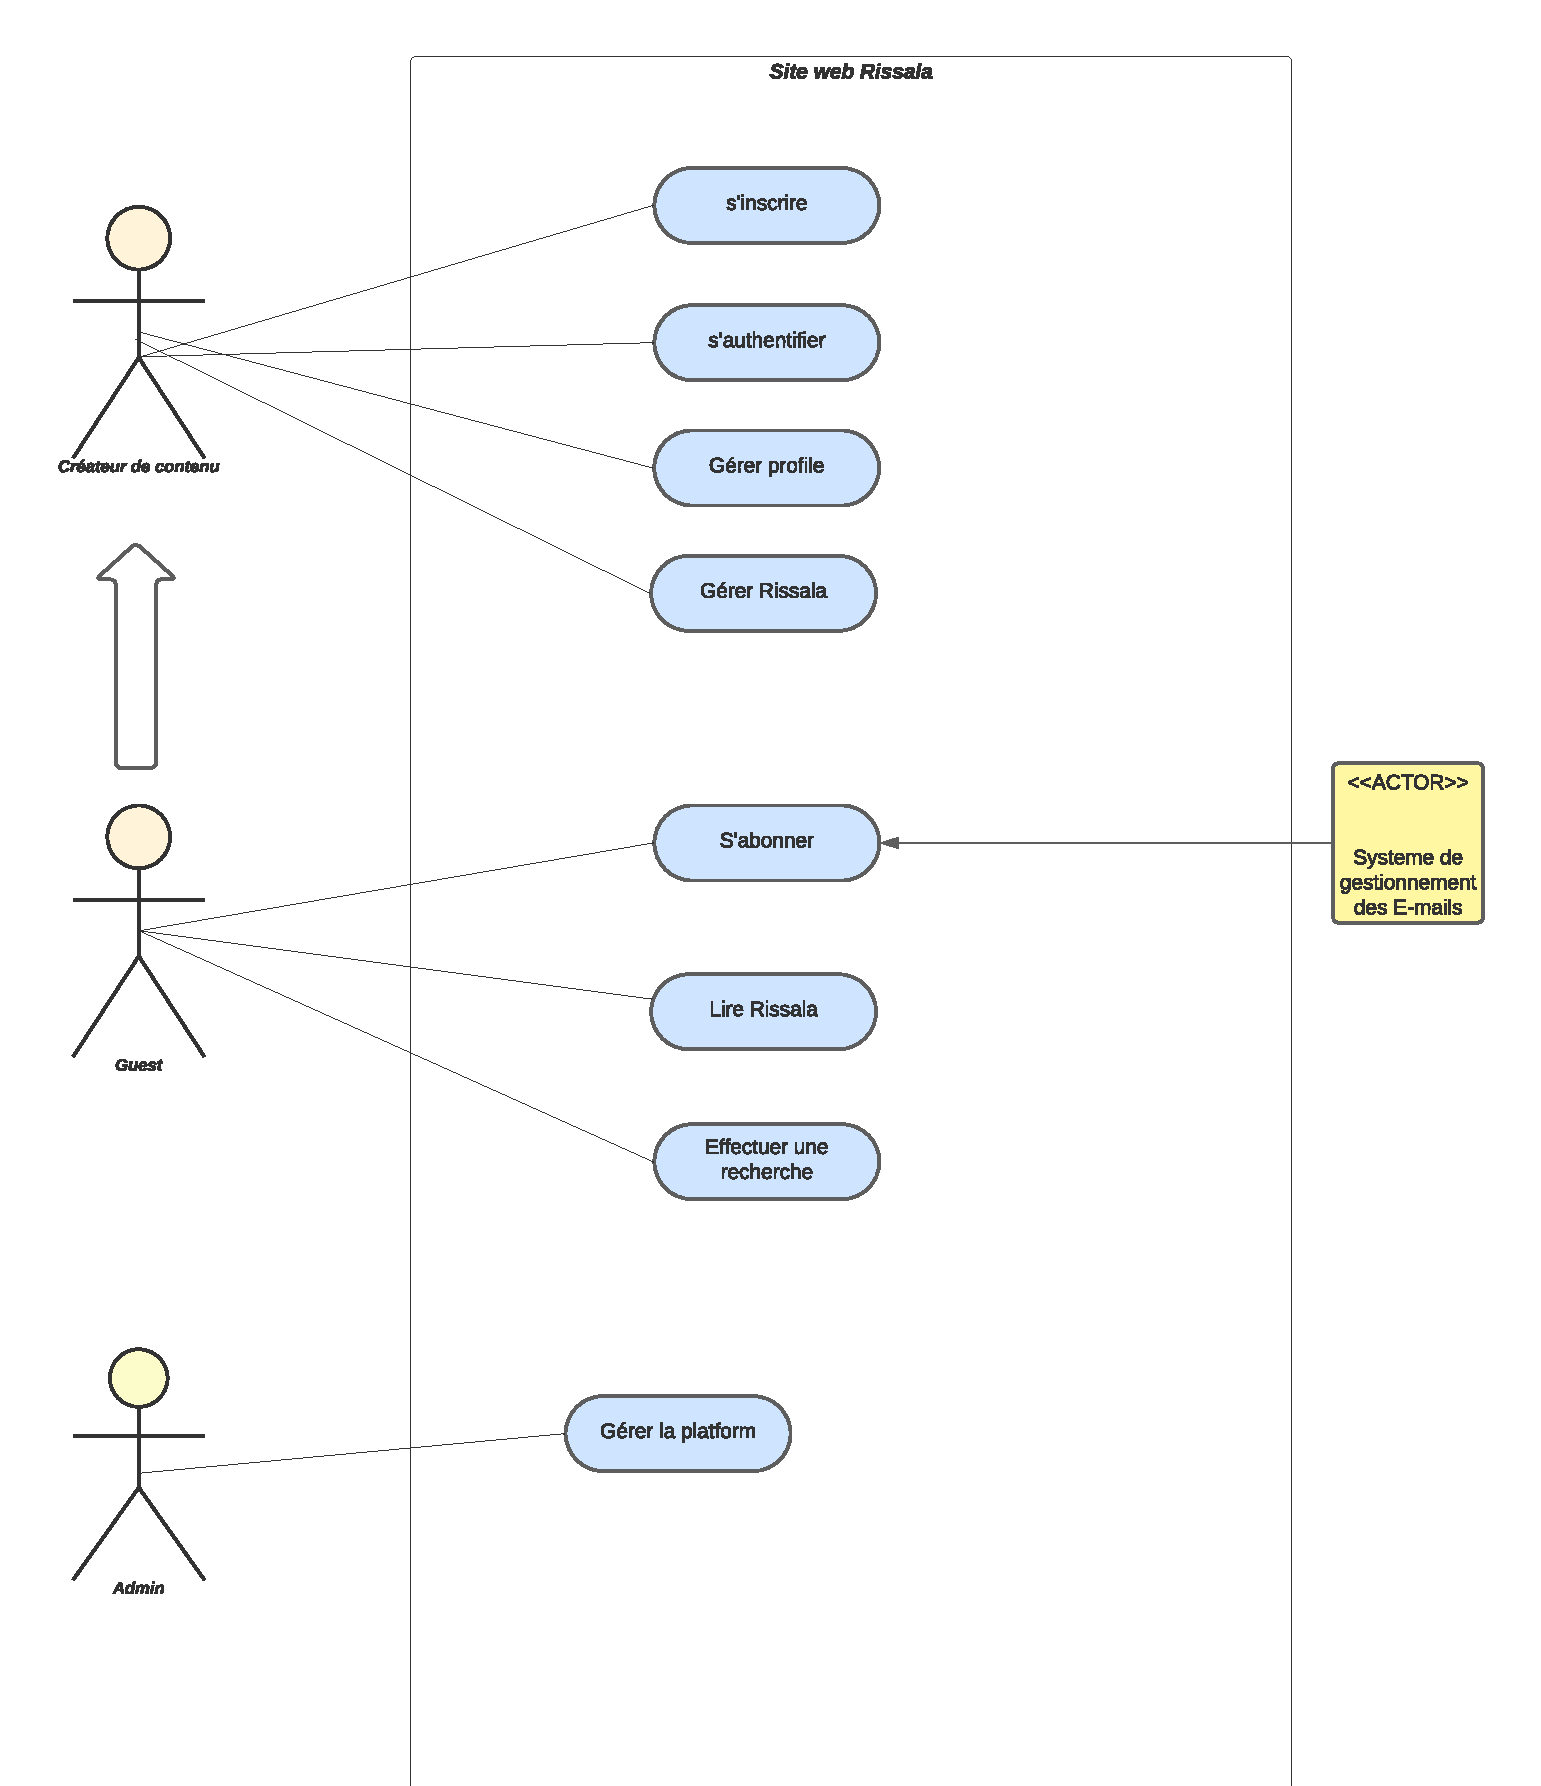
\includegraphics[width=1.\textwidth,height=1.5\textheight,keepaspectratio]{image/Diagramme vierge.pdf}
    \caption{Diagramme du cas d'utilisation n*1}
    \label{fig:diagramme}
\end{figure}
\chapter{Les Interfaces}
Pour une consultation plus précise des interfaces, veuillez vous référer à notre projet sur Figma.
\url{https://www.figma.com/file/qPQb27LuO5XC7c0dZNxZG4/Rissala-Project-UI?type=design&node-id=0-1&mode=design&t=kXxYedrESPdWnNO0-0}
section{les privilèges de chaque acteur}
\subsubsection{Admin}
L'administrateur a le privilège de gérer l'intégralité de la plateforme.



\subsubsection{Le créateur de contenu}
En tant que créateur de contenu, il est nécessaire de se connecter pour accéder à son profil et créer des newsletters. Par ailleurs, vous avez la possibilité de consulter les newsletters créées par d'autres utilisateurs, comme illustré dans le diagramme du cas d'utilisation. 
\subsubsection{guest}
En tant qu'invité, vous avez la possibilité de rechercher des newsletters, de vous y abonner, de consulter les newsletters ainsi que les créateurs de contenu.
\section{interfaces}
\clearpage
\begin{figure}[htbp]
    \centering
    \begin{minipage}[b]{0.7\textwidth}
        \centering
        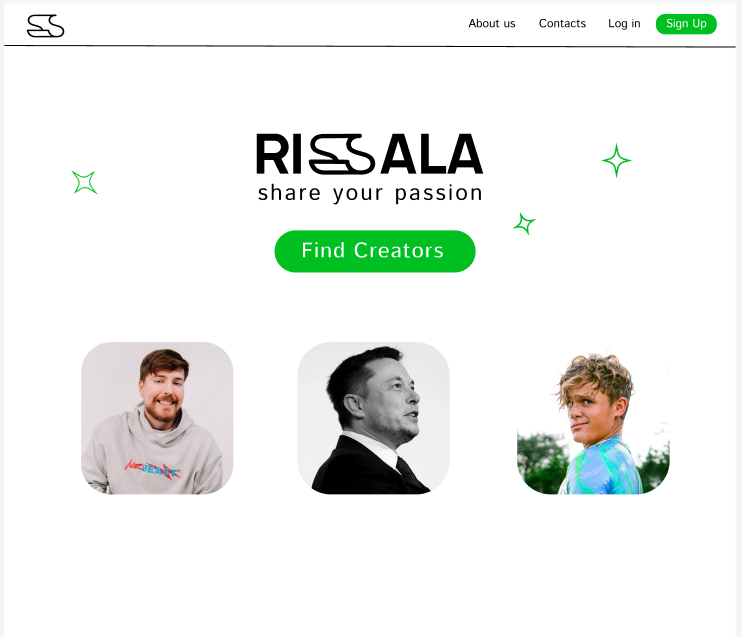
\includegraphics[width=\textwidth]{interfaces/index.png}
        \caption{Index}
        \label{fig:index}
    \end{minipage}
    \hfill
    \begin{minipage}[b]{0.7\textwidth}
        \centering
        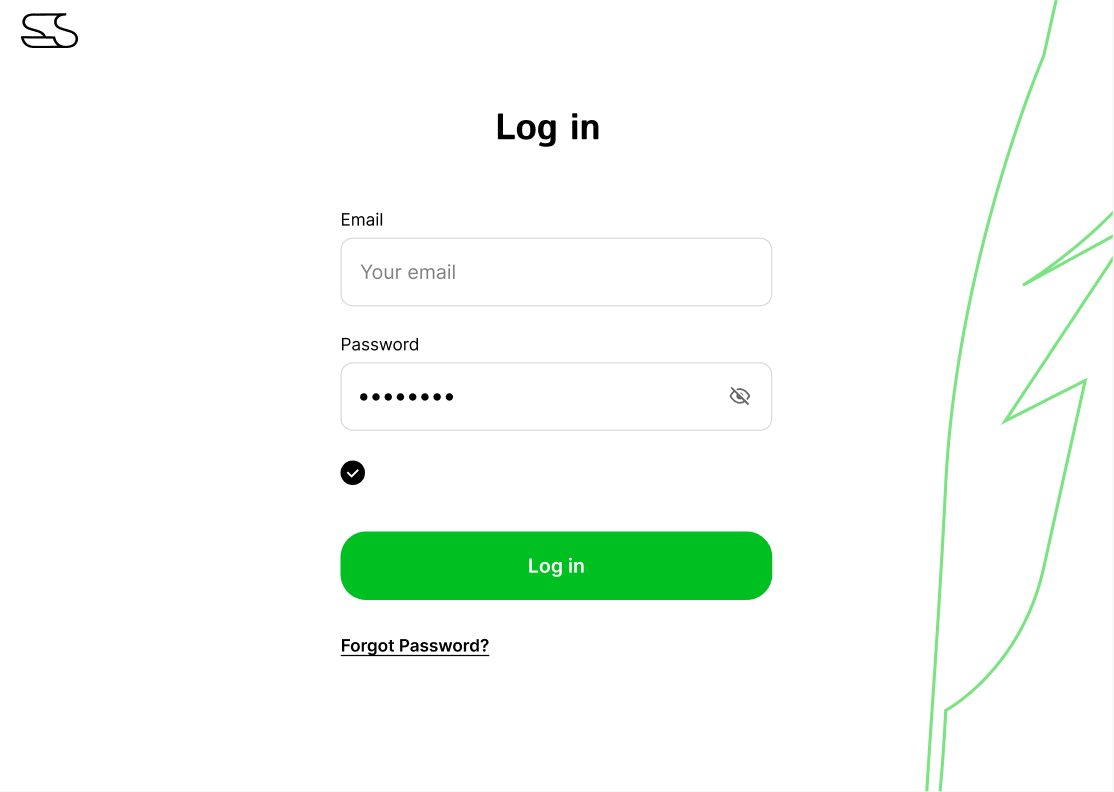
\includegraphics[width=\textwidth]{interfaces/log in.png}
        \caption{Log in}
        \label{fig:connexion}
    \end{minipage}
\end{figure}
\begin{figure}
    \centering
    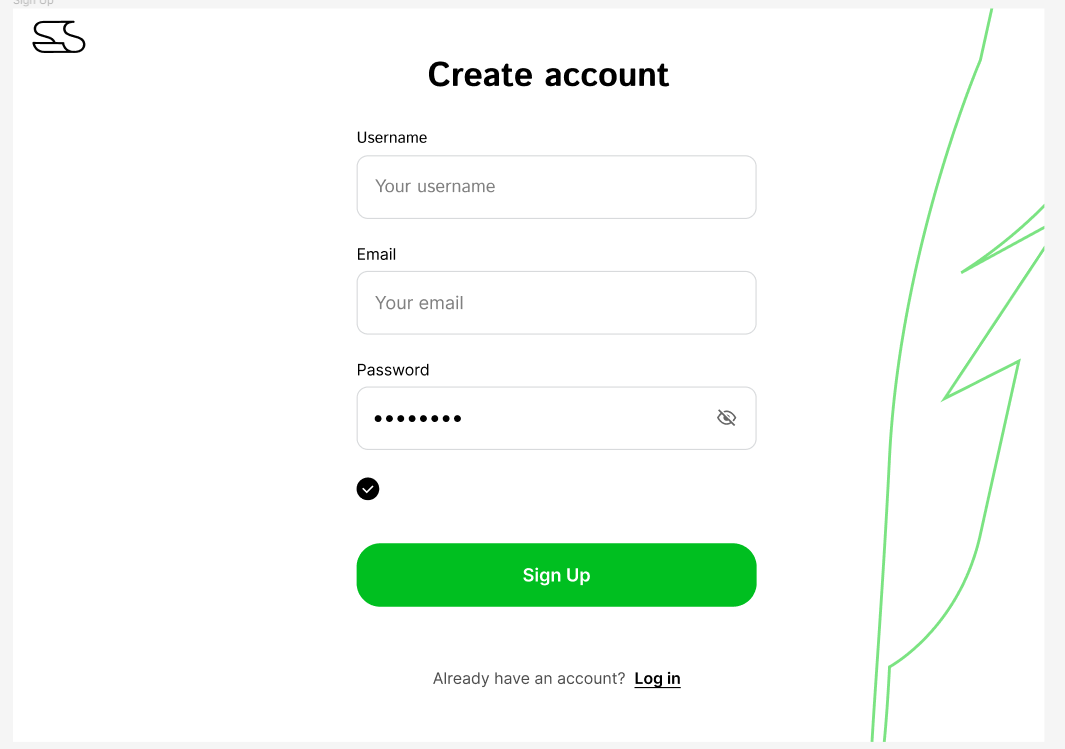
\includegraphics[width=0.7\textwidth,height=1\textheight,keepaspectratio]{interfaces/sign up.png}
    \caption{Sign in}
    \label{fig:diagramme}
\end{figure}
\begin{figure}
    \centering
    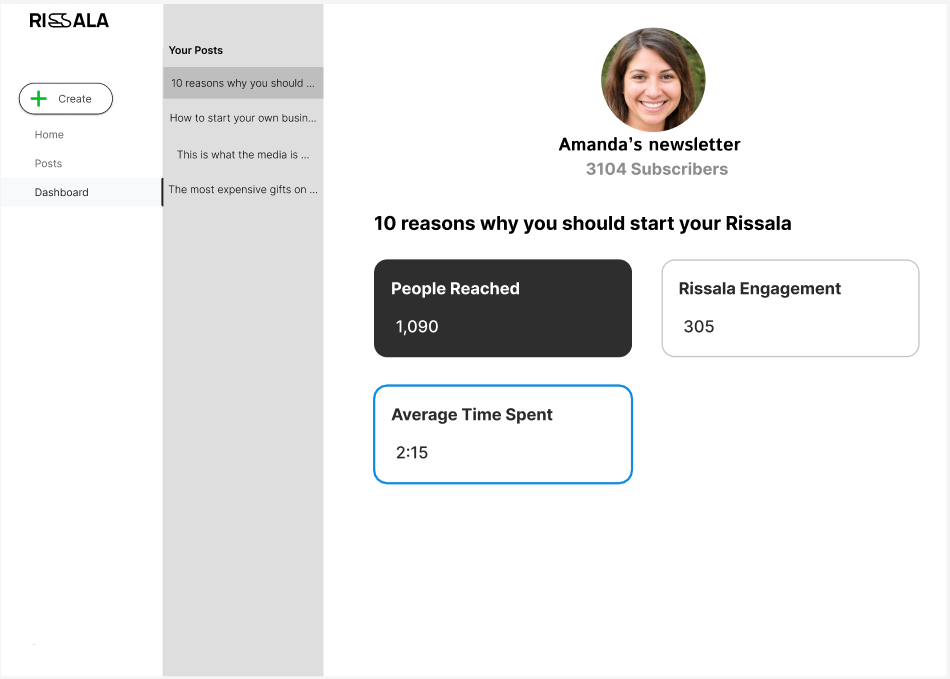
\includegraphics[width=0.7\textwidth,height=1\textheight,keepaspectratio]{interfaces/Dashboard.png}
    \caption{Dashboard}
    \label{fig:diagramme}
\end{figure}
\begin{figure}
    \centering
    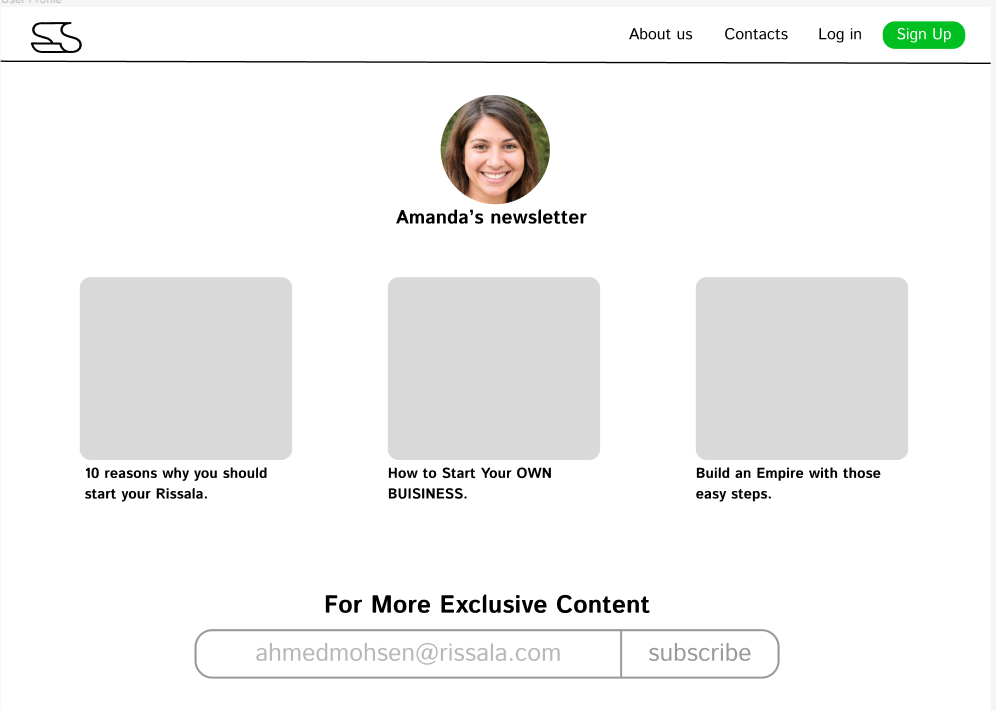
\includegraphics[width=0.7\textwidth,height=1\textheight,keepaspectratio]{interfaces/user profile.png}
    \caption{Profile}
    \label{fig:diagramme}
\end{figure}
\begin{figure}
    \centering
    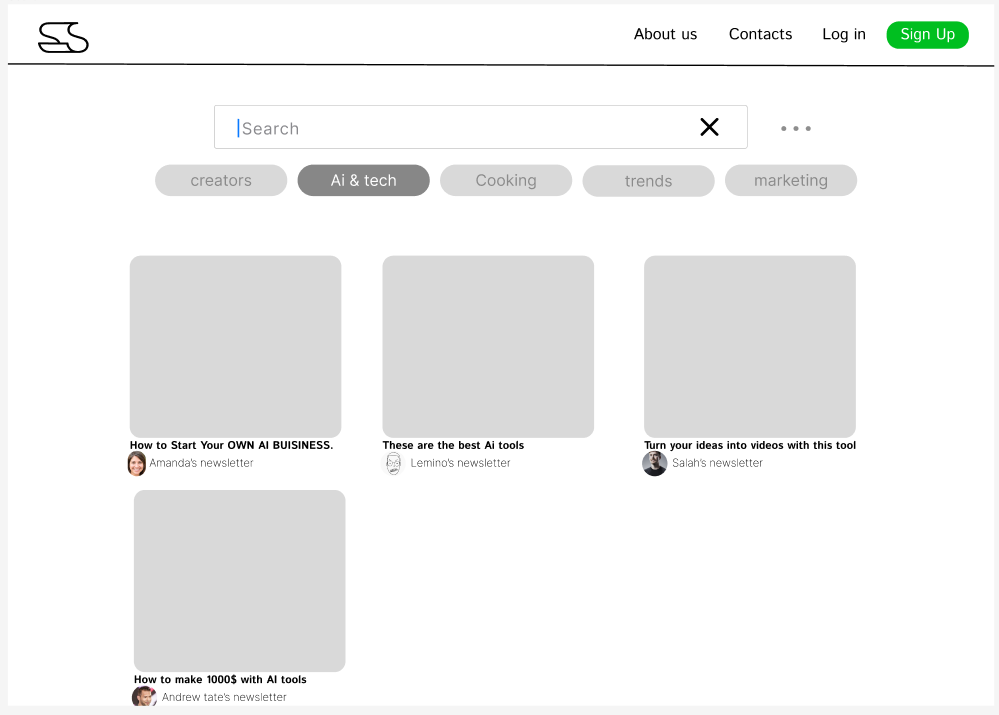
\includegraphics[width=0.7\textwidth,height=1\textheight,keepaspectratio]{interfaces/search.png}
    \caption{Search}
    \label{fig:diagramme}
\end{figure}
\begin{figure}
    \centering
    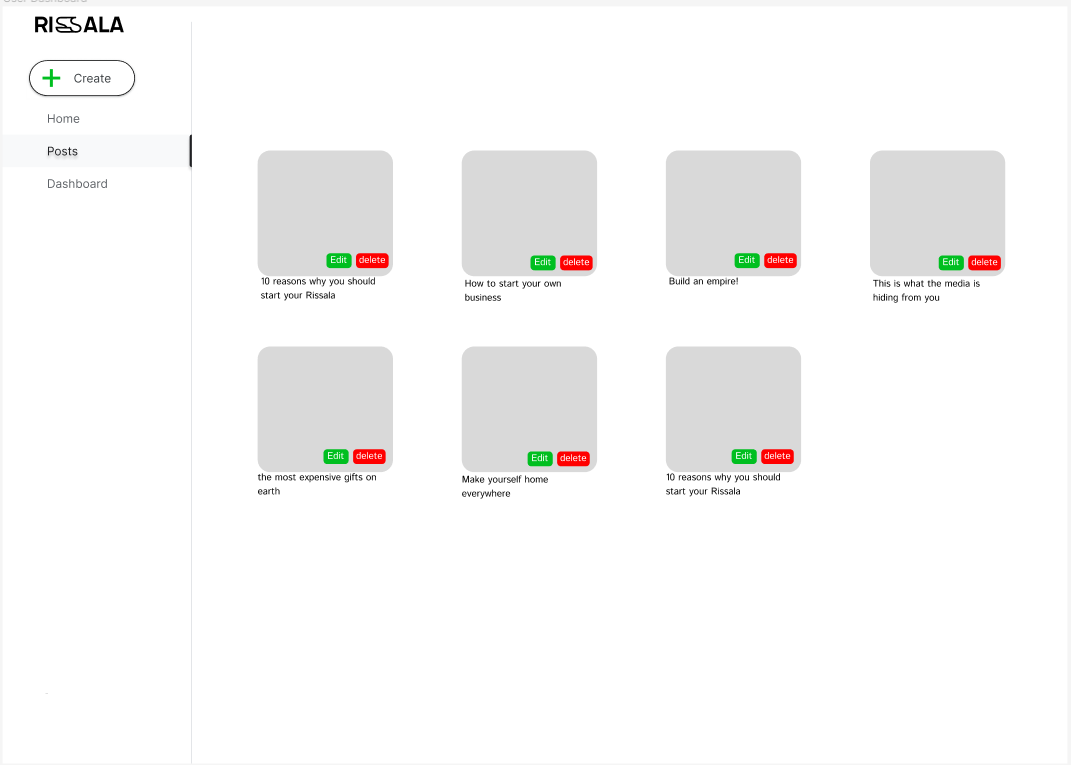
\includegraphics[width=0.7\textwidth,height=1\textheight,keepaspectratio]{interfaces/posts.png}
    \caption{Postes}
    \label{fig:diagramme}
\end{figure}






\end{document}